\documentclass{aamas2018}

% We invite submission of original work, up to 8 pages in length

\pdfpagewidth=8.5truein
\pdfpageheight=11truein

\usepackage{graphicx}                                        % for eps, pdf, jpeg, png and tif graphics
\usepackage{amsmath}                                         % for align
\usepackage{amssymb}                                         % for >= and <= signs
\usepackage{xfrac}                                           % for nice x/y fractions (sfrac)
\usepackage{tikz}
\usepackage{amsbsy}                     % for boldsymbol
\usepackage{upgreek}

\mathchardef\mhyp="2D    % define math mode hyphen

\allowdisplaybreaks[4]

\title{A deep feedback learning architecture which employs error forward propagation}

\numberofauthors{2}

\author{
% You can go ahead and credit any number of authors here,
% e.g. one 'row of three' or two rows (consisting of one row of three
% and a second row of one, two or three).
%
% The command \alignauthor (no curly braces needed) should
% precede each author name, affiliation/snail-mail address and
% e-mail address. Additionally, tag each line of
% affiliation/address with \affaddr, and tag the
% e-mail address with \email.
% 1st. author
\alignauthor
Bernd Porr\\
       \affaddr{Glasgow Neuro LTD}\\
       \affaddr{Glasgow, United Kingdom}\\
       \email{bernd@glasgowneuro.tech}
% 2nd. author
\alignauthor
Paul Miller\\
       \affaddr{Glasgow Neuro LTD}\\
       \affaddr{Glasgow, United Kingdom}\\
       \email{paul@glasgowneuro.tech}
}


\begin{document}

\maketitle

\begin{abstract}
  Deep networks so far have been developed on the basis of an error
  signal being generated by comparing the output to some desired
  value, and then propagating this signal backward through the
  network. However, autonomous agents define their errors at the
  \textsl{inputs} by reference to a desired or expected state. This is
  because they act as a closed loop system and not open loop. This
  calls for a network where the error is propagated from its input to
  its output and where the feedback from the environment propagates it
  back to its input. In this paper we present a novel learning
  algorithm which performs ``forward-prop'' of the error in parallel
  to the activation. This approach is in line with both neuroscience,
  and the philosophy behind closed loop systems. We demonstrate its
  performance, first in a simple line follower, and then in a first
  person shooter game.
\end{abstract}


 \begin{CCSXML}
<ccs2012>
<concept>
<concept_id>10003752.10010070.10010071.10010289</concept_id>
<concept_desc>Theory of computation~Semi-supervised learning</concept_desc>
<concept_significance>300</concept_significance>
</concept>
</ccs2012>
\end{CCSXML}

\ccsdesc[300]{Theory of computation~Semi-supervised learning}


\printccsdesc


%Keywords are your own choice of terms by which you would like the paper to be indexed.

\keywords{Hebbian learning, heterosynaptic learning, deep learning, neural network, closed loop, autonomous behaviour, feedback, error signal}


\section{Introduction}
When an agent acts in its environment, its actions in turn will change
its sensor inputs which in turn will cause new actions -- in short,
the agent acts in a closed-loop system. In the simplest case this is a
reactive system where the agent encounters threats or rewards and acts
accordingly. Both threats and rewards are unpredictable events where
the agent must respond as quickly as possible. These are often called
``disturbances'' \cite{Phillips2000} or
``perturbations'' because they force the agent to
act at an unpredictable moment in time. Importantly, these occur at
the \textsl{input} of the agent and, thus, a closed loop system
performs ``input control'' \cite{Phillips2000} -- in contrast to a pattern recognition
system which performs ``output control''
\cite{Phillips2000,Porr2005kyb}.

The above scenario has a major drawback in that the reactions are
always too late. It would be safer for an agent to learn to predict
these disturbances from other cues and pre-empt them, thereby
introducing the concept of adaptive behaviour. At the moment of the
disturbance it's already too late - the tiger has already attacked, or
the food has been found by pure coincidence. However, one can then
look back in time and determine which input signals could have
predicted this unexpected threat or reward
\cite{Sutton87,Sutton98,Abbott01,NIPS2002_2245,PorrNecoInvco2003}.

Adaptive controllers for this kind of learning are either
correlation-based \cite{Klopf86,PorrNecoISO2003,Verschure91} or state
space-based \cite{Dayan1992,Sutton98}. The state space-based ones can
become very powerful by utilising a deep learning network
\cite{Guo2014}. However, the deep learning architecture requires backprop which
is an open loop algorithm, and can only be used by embedding the
network into traditional Q/RL learning
paradigms \cite{Dayan1992,Guo2014}. On the other hand correlation
based-methods can be very fast \cite{Porr2006ICO}, but so far it has
been difficult to use them directly on deep networks. These
correlation based methods use ``input control'', which means that the
error signal is fed into the network at its inputs.

For nearly a century Neurophysiology has also supported a forward
propagation mechanism which has first been proposed theoretically by
Hebb \cite{Hebb49}, and then confirmed many times: for long term
potentiation (LTD) to happen, both pre- and post-synaptic neurons need
to be active \cite{Luescher2012}.  There has been a long tradition of
work showing that unsupervised learning is possible in these networks
\cite{Linsker88}, in particular in the visual cortex \cite{Miller00}
in an open loop fashion. However, here we are in the realm of
reinforcement learning, which is closed loop. One solution is to
introduce direct feedback to mimic backprop \cite{Lillicrap2016}, but
this will fail in deeper architectures, and requires additional
assumptions which are not biologically realistic.  However, there is
emerging evidence that different brain oscillations can carry separate
information via the same neurons, which allows for transmission of separate
streams through the same networks in a forward fashion
\cite{Mizuhara2007,Canolty2010}. Disruption has been linked to
various mental illnesses \cite{Kim2016,Won2017}. These different
streams of activity are not just carrying different kind of
information, but also have different impacts on plasticity, with the
higher frequency components most likely altering plasticity as shown
in high frequency stimulations (HFS) \cite{Bliss73}, and the lower
ones relevant for behaviour or mental processes while keeping
plasticity constant \cite{Mizuhara2007}.

How could an error be propagated through a deep network in a forward
fashion? Here we take inspiration from how errors are transmitted in
backprop. In essence the hidden layers receive a \textsl{weighted sum}
of the errors from the previous layers, which makes intuitive sense:
the strongest weights contribute the most to the error. Imagine we
take a similar approach using forward propagation: the error,
introduced at the input, will have its strongest impact via the
largest weights. Therefore we propagate the error in a forward fashion
in the same way as in backprop. Eventually the agent will make an
action and this will feed back to the input of the agent, which then
in turn corrects the weights in all layers.

In this paper we present a novel deep network algorithm for closed
loop systems which we call ``Deep Feedback Learning'' (DFL). This
algorithm marries the ideas for correlation based closed loop learning
with those from deep learning, by turning deep learning from a
backprop-based algorithm to a forward-prop one. We demonstrate this
with two scenarios: a driving task and a 1st-person shooter.

\begin{figure}[!ht]
  \centering
  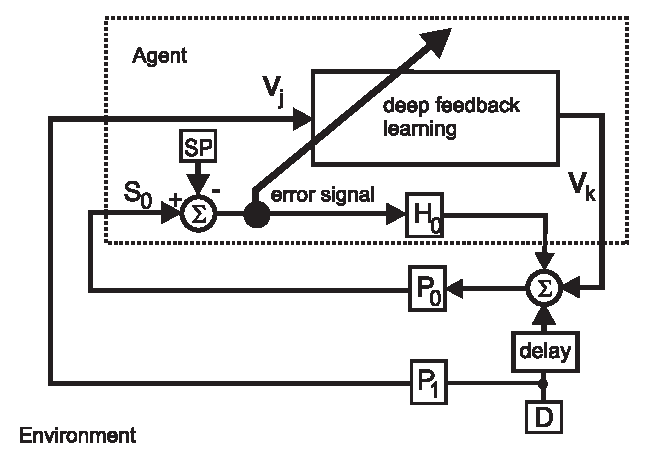
\includegraphics[width=0.9\columnwidth]{closed_loop}
  \caption{A closed loop system with a setpoint $SP$, transfer function $H_0$ and the
    environment $P_0$ which needs to work against unpredictable disturbances $D$.
    The error signal tunes a deep neuronal network, which has inputs
    $v_j$ that predict the disturbances. The network tries to pre-empt these
    disturbances and generate an appropriate action $v_k$.
    \label{closed_loop}}
\end{figure}

\section{Closed loop learning}
Before we describe the algorithm, we need to place it in a closed loop
context. Fig.~\ref{closed_loop} shows the entire closed loop system
with the deep feedback learning as a black box for now. The idea is
that we have a fixed closed loop which is able to fend off
disturbances, such as an unexpected bend on a road or the sudden
appearance of an enemy. This fixed loop then takes appropriate action
to solve this disturbance, e.g. correcting a car's steering, or aiming
towards and shooting an enemy. In formal terms we have a setpoint $SP$
which compares the input of the organism to a desired input. If the input
deviates from the setpoint an action is generated with the transfer
function $H_0$. This action then eliminates the disturbance $D$ and
arrives via the environmental transfer function $P_0$ at the input
again; thus, the loop is closed. However, we are not so much
interested in the design of the closed loop but rather that it
generates an \textsl{error signal}. This error signal is non-zero if a
disturbance has happened, and can be used to tune our deep feedback
learning network.

The deep feedback learning network receives additional inputs which are able
to predict the disturbance, and thus prevent the trigger of the feedback
loop. These additional inputs are provided via the transfer function $P_1$
and represent the disturbance in a filtered form. For example a video camera
can provide images of the road ahead, or of an enemy. Deep feedback
learning has the task to take the error signal, and tune its network
to generate actions to minimise the error. In the next section
we describe the deep feedback learning and how this can
compute the appropriate output.

\begin{figure}[!ht]
  \centering
  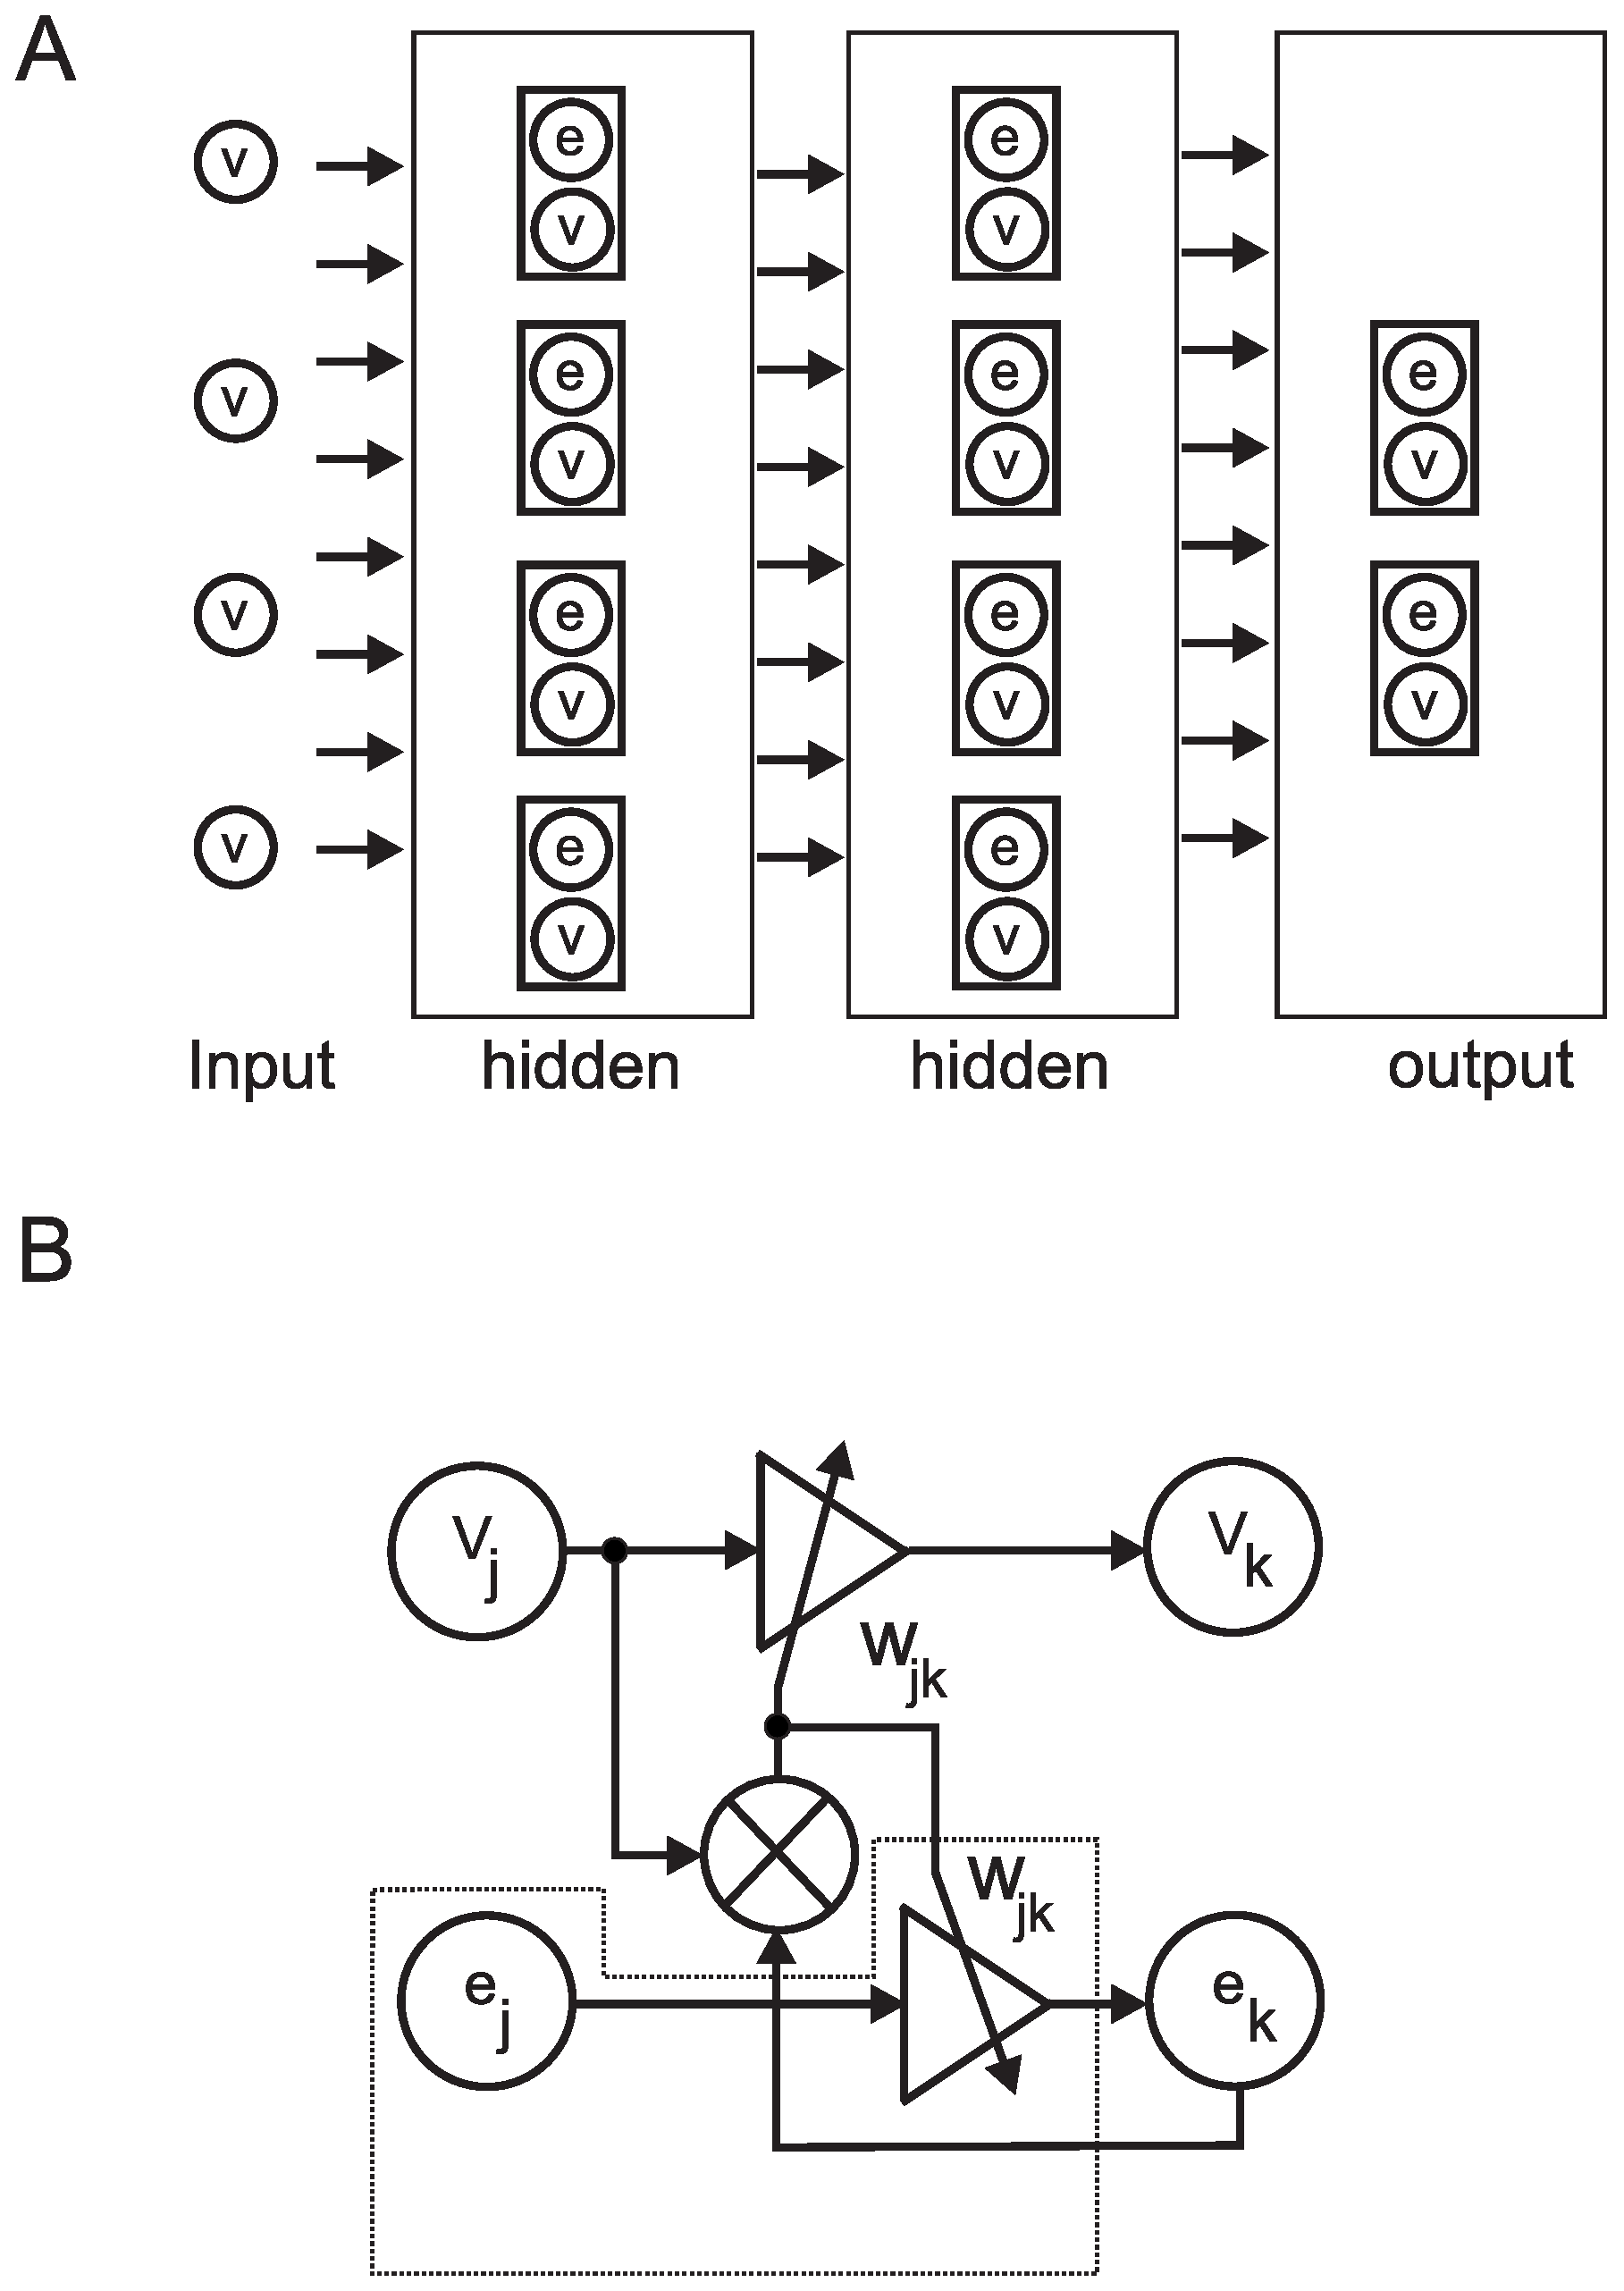
\includegraphics[width=0.75\columnwidth]{netw_together}
  \caption{A) Network overview. With the exception of the input layer, every
    neuron is a composite cell with an activation $v$ and an error
    term $e$. These are propagated through the network in a weighted
    fashion in parallel.  B) Computation in a single composite cell.
    The presynaptic activities $v_j$ and error signals $e_j$ are used
    to perform correlation based learning and change the weight
    $w_{jk}$ which has the same value for both error and activation.
    The dotted box is only implemented in the deeper layers but not
    in the input layer which receives its error signal from the reflex loop.
    \label{netw_together}}
\end{figure}


\section{Deep feedback learning}
We define a network with an input layer, hidden units and an output
layer which can all have different numbers of neurons (see
Fig~\ref{netw_together}A). In contrast to traditional
networks, every layer (except for the input layer) consists of two
summation nodes: the actual activity and an error signal. These
are processed in two parallel streams.

Let us first focus on the network activity. We define a multi-layered
network, where every neuron is a standard computational unit that
calculates a weighted sum $v_k$ of its inputs $v_j$ and then applies
an activation function $\Theta(v) = \tanh(v)$:
\begin{equation}
  v_k = \Theta\left( \sum_j w_{jk} v_{j} \right) \label{act_sum}
\end{equation}
where the activity flows from neurons in layer $v_j$ to neurons in
layer $v_k$ multiplied by the weights $w_{jk}$, and this
is then repeated in the next layer. This means that for a network with
$N$ layers we have $N-1$ sets of weights $w_{jk}$.

The weight changes are then updated in a semi-Hebbian fashion:
\begin{equation}
  w_{jk}(t+1) = w_{jk}(t) + \gamma v_j(t)  e_k(t) + \mu w_{jk}(t) \label{learningRule}
\end{equation}
where $v_j(t)$ is the presynaptic activity and $e_k(t)$ is an error
signal attached to the postsynaptic neuron, so the correlation is
calculated between input signals and the error signal with the
standard parameters learning rate $\gamma$ and momentum $\mu$.

We now describe the error signal propagation. As outlined above, the
error signal emerges from the feedback loop, and is injected into the
network at its 1st hidden layer as the ``postsynaptic'' activity. The
weight change for this 1st layer can then be calculated directly with
Eq.~\ref{learningRule} by setting $e_k$ to the error signal of the
feedback loop (see Fig.~\ref{closed_loop}).

For the deeper layers, the error signal is computed as a weighted
sum of the error signals from the previous layer:
\begin{equation}
  e_k = \frac{\left( \sum_j w_{jk} e_{j} \right) \Theta^\prime (v_k) }{\frac{\sum_j {|w_{jk}|}}{\sum_j 1}}
  \label{deepError}
\end{equation}
where the $\Theta^\prime (v) = 1 - v^2$ is the derivative of the
activation function $\Theta(v)$: this limits learning when the unit
approaches saturation, as in backprop. The norm guarantees that
the error propagates through all layers and does not vanish from
layer to layer due to small weights.

A simplified data flow diagram of the learning performed in each layer
is shown in Fig~\ref{netw_together}B, where we see the two processing
streams: both the activity $v_j$ and error signal $e_j$ are weighted
by $w_{jk}$, and summed separately in the next layer. Remember that
for the 1st hidden layer, the error is just the error signal
directly injected from the feedback loop. The diagram omits the error
normalisation, scaling and activation derivative in order to focus on
the main point that learning happens between the error signal and the
presynaptic activity.

Learning is then performed in three steps: first the activity is
propagated through the network, then the error signal is propagated
via the same mechanism, and finally the weights are adjusted. Thus,
both the error signal and the activity is propagated in a forward
fashion. Learning itself can be interpreted as heterosynaptic for the
activity $v_j$ and Hebbian for the error $e_j$.


\begin{figure}[!ht]
  \centering
  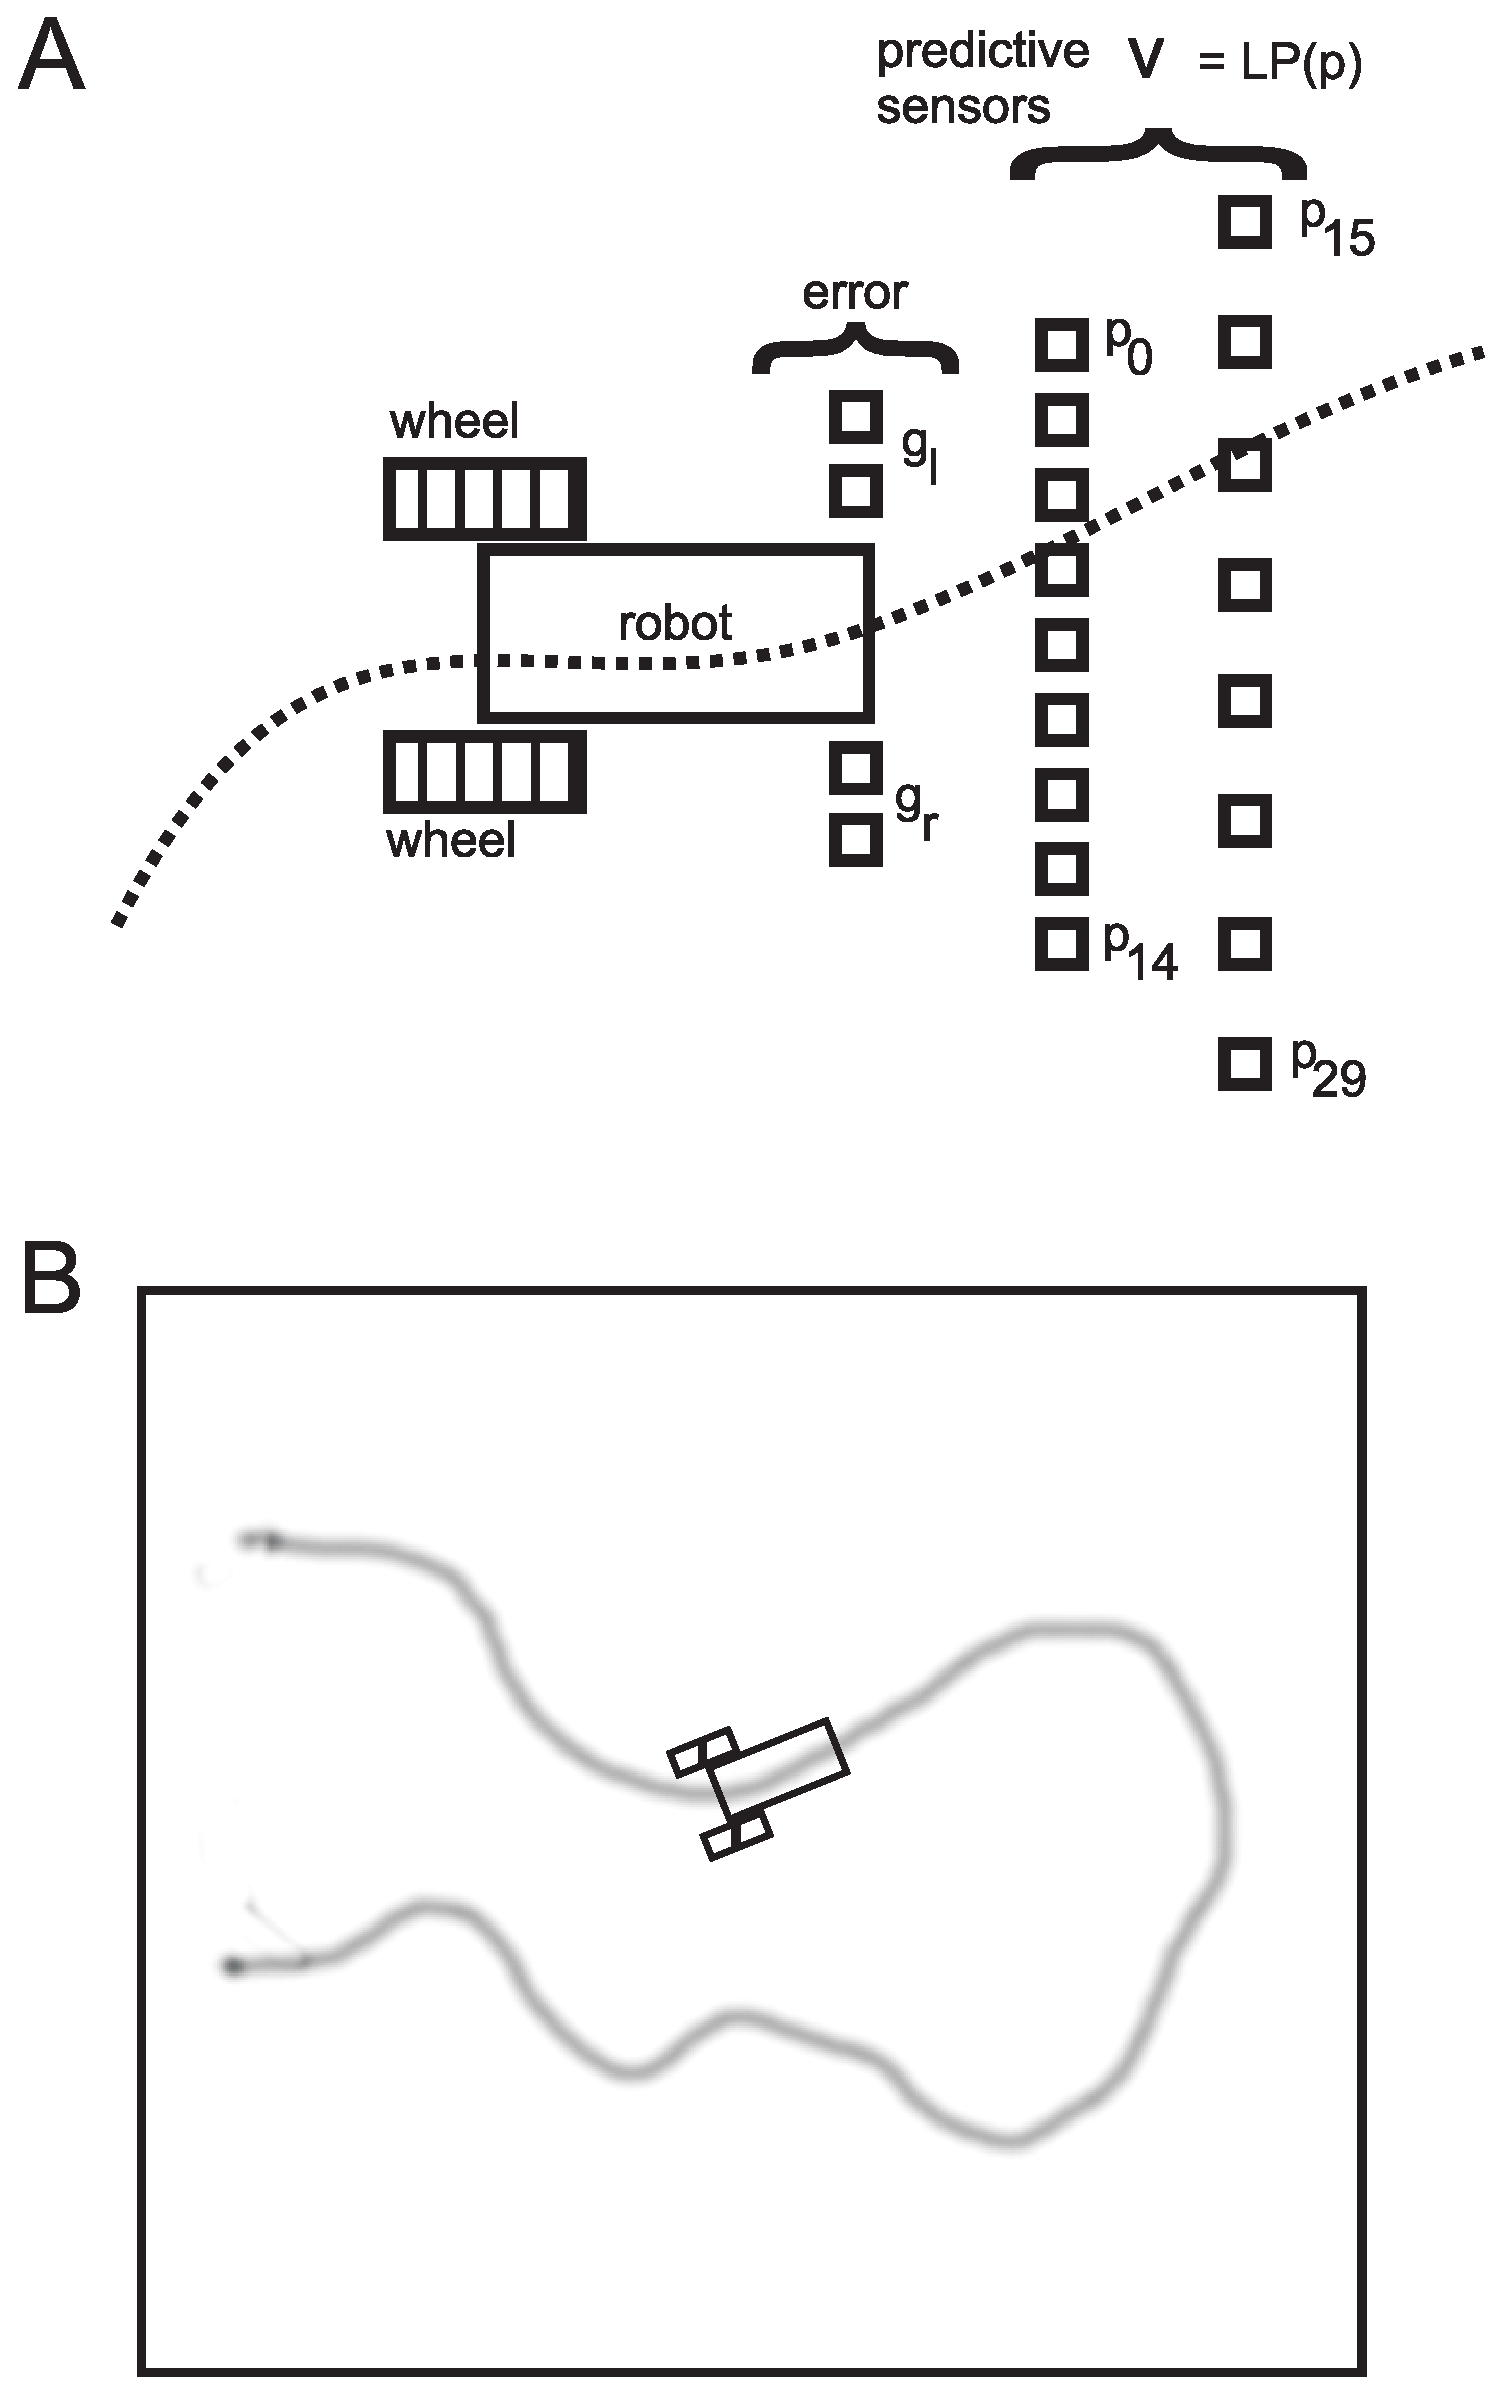
\includegraphics[width=0.85\columnwidth]{linefollower_robot_playground}
  \caption{A) Robot setup. The robot is simulated with a updated
    version of enki for QT5 (\texttt{https://github.com/glasgowneuro/enki})
    where the line follower is using just the ground sensors of the
    robot to create the error signal ($g_l$, $g_r$) and the predictive signals ($p_m$)
    for DFL. Each of the 30 predictive signals $p_m$ from the two rows of ground sensors
    is split into 10 2nd-order lowpass filters with impulse responses
    lasting from $2$ to $30$ timesteps, and then these all feed into the DFL
    network as predictive inputs $v_j$, giving 300 inputs in total.
    The robot has two wheels whose speed is controlled
    by the feedback control and DFL.
    B) The line following scenario used for the simulations. The robot
    attempts to drive along the line and is reversed at the end of the
    line and then drives back. If it hits the boundaries of the playground
    it is also turned around.
    \label{linefollower_robot_playground}}
\end{figure}

\begin{figure*}[!ht]
  \centering
  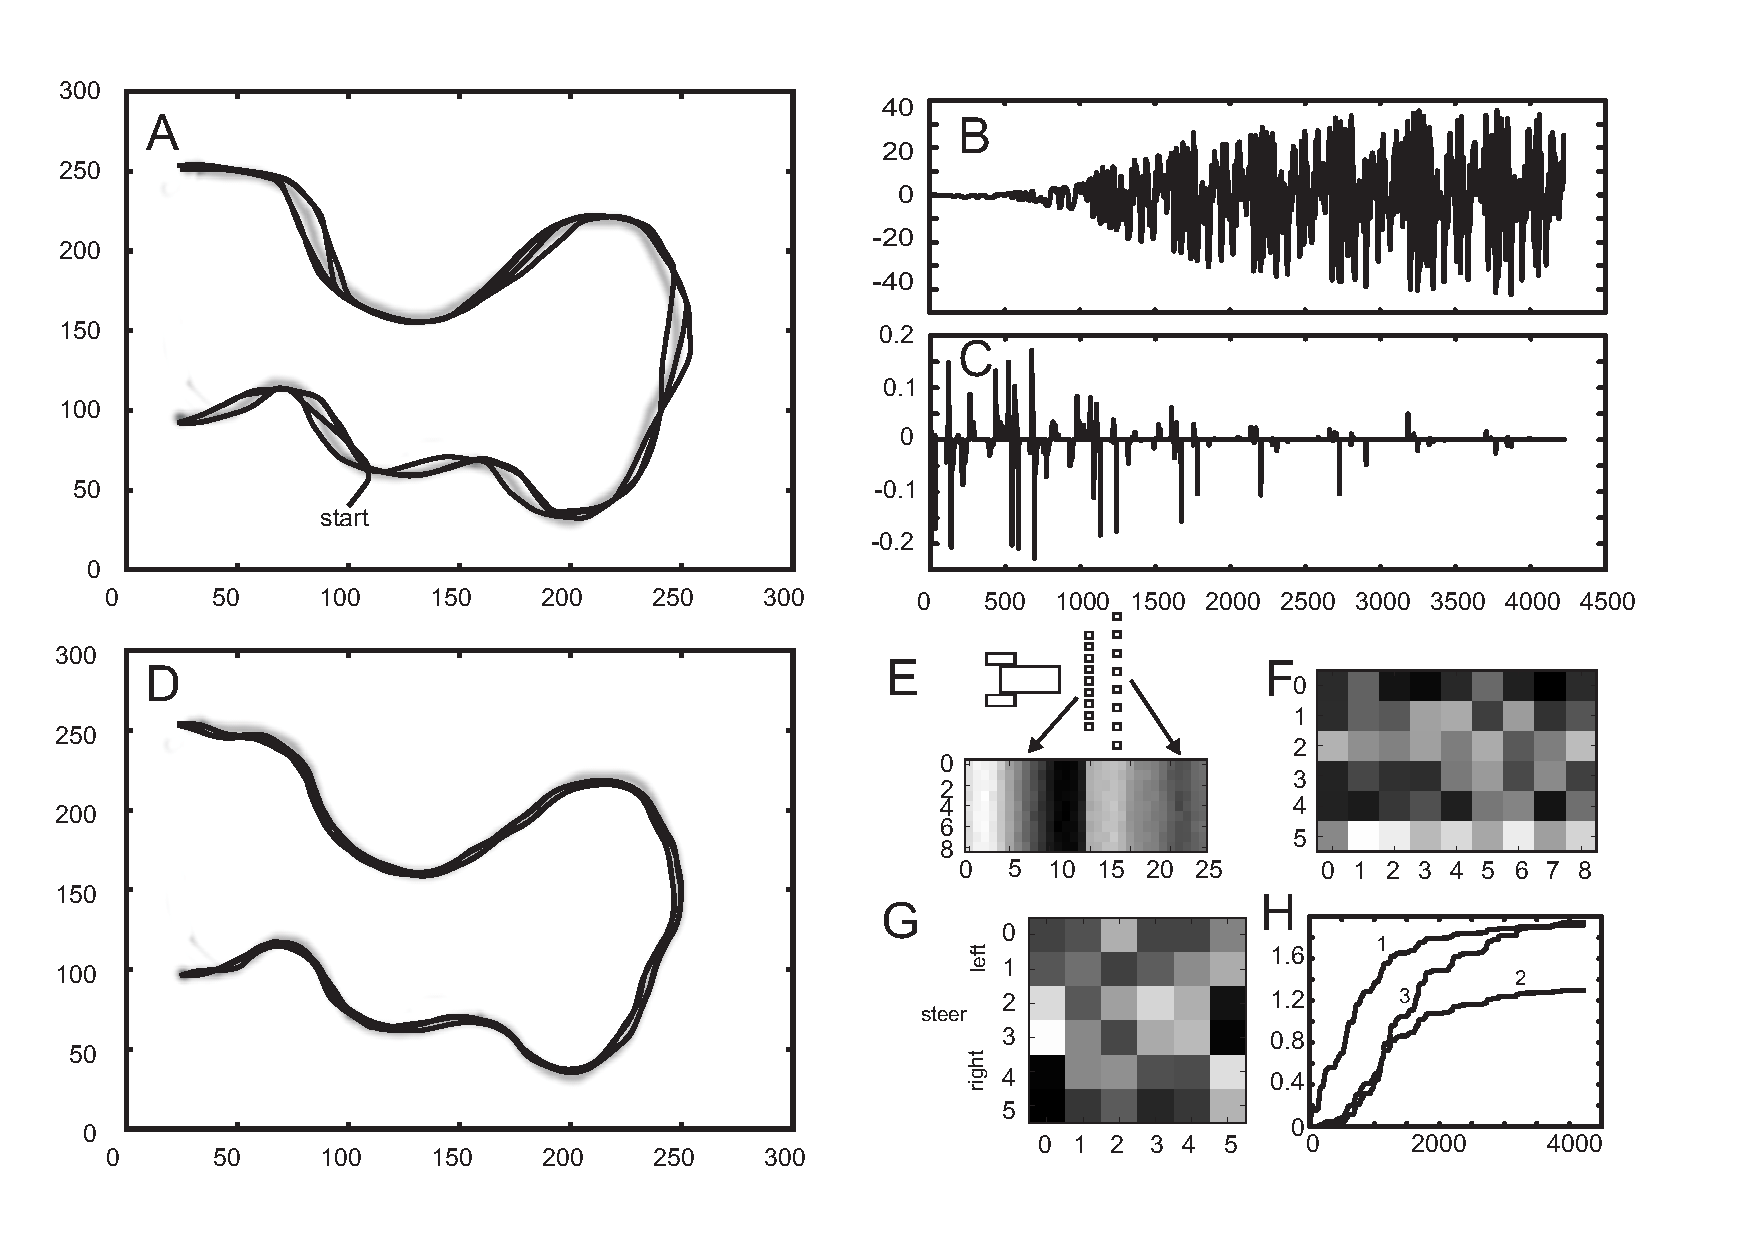
\includegraphics[width=\linewidth]{line_results}
  \caption{Results of the line following task. A) shows the robot at
    the very start of the simulation run from time step 0 to 1000. B)
    the difference between the robot wheel speeds just for the learned
    actions (i.e. the output of the DFL network): $v_l-v_r$.  C) the
    error signal.  D) simulation run just before the final 1000 time
    steps where the absolute value of the error has been below 0.001
    for 1000 time steps. E-G) show the weights of the different
    layers. The input neurons are on the x-axis and the output neurons
    are on the y-axis.  E) the weights of the 1st layer, F) the
    weights of the 2nd layer and G) the weights of the output layer.
    H) shows the euclidean distance of the weights for each layer from
    their random work initialisation. Parameters: 30 inputs from two
    predictive rows of sensors (15 each). Every input was fed into a
    filterbank of 10 filters with T=2 \ldots 30. There were 2 hidden
    layers with 9 and 6 neurons; 6 output neurons. The learning rate $\gamma$
    was 0.0001 and the momentum $\mu$ was set to 0.9. Learning was disabled
    when the robot turned to avoid large error spikes caused by the learning
    and the error was also set to zero during turning.
    \label{line_results}}
\end{figure*}








\section{Line follower}
In order to demonstrate and benchmark DFL we need a simple closed loop scenario
which can be improved with the help of an adaptive network.
Fig.~\ref{linefollower_robot_playground} shows a simple line following
robot which has the task of following the line depicted in
Fig.~\ref{linefollower_robot_playground}B to the end, where it
reverses and drives back, and so on. The four ground sensors in
Fig.~\ref{linefollower_robot_playground}A left/right on either side
of the robot create an error signal:
\begin{equation}
\mathrm{error} = (g_{l_1}+2 g_{l_2})-(g_{r_1}+2 g_{r_2}) \label{line_error}
\end{equation}
this error directly creates a steering reaction from the fixed
feedback loop by controlling the speed of the wheels.

The DFL learning circuit uses the predictive ground sensors - these
are first filtered by a filterbank, which smears them in time and
creates a temporal overlap with the error signal. These filtered
signals are then presented to the $v_j$ of the input layer (see
Eq.~\ref{act_sum}). We have two rows of sensors, one directly in front
of the robot and one which looks further ahead. There are 30 ground
sensors each filtered by 10 filters, giving 300 inputs in total.

The output layer of our deep feedback learner consists of 6 neurons
with activations $v_k$ ($k=0 \ldots 5$) - these can be seen as soft
decision-making units where 3 of them determine the change of speed of
the right wheel, and 3 the left wheel. This leads to the
final formulas for the motor outputs:
\begin{eqnarray}
  \mathrm{leftSpeed} &=& s_0 + \underbrace{g\, \mathrm{error} + \left( 50 v_0 + 10 v_1 + 2 v_2 \right)}_{v_l} \\
  \mathrm{rightSpeed} &=& s_0 - \underbrace{g\, \mathrm{error} + \left( 50 v_3 + 10 v_4 + 2 v_5 \right)}_{v_r}
\end{eqnarray}
where $v_0, \ldots, v_5$ are the 6 outputs from the DFL network. Note
that neither inputs nor outputs are organised in a topographically
meaningful way. The network must discover from the error signals
which sensor inputs $v_k$ will eventually lead to appropriate steering
actions. At the start the network is initialised with random values.

As performance criterion we use the absolute value of the error from
Eq.~\ref{line_error}:
\begin{equation}
  \mathrm{error}_\mathrm{abs} =  |\mathrm{error}| \label{line_abserr}
\end{equation}
which needs to be below a threshold of $0.001$ for 1000 time steps
because realistically, driving will never be 100\% perfect, and we
allow $\mathrm{error}$ to stabilise at small values.


\subsection{Results}
Fig.~\ref{line_results} shows the results of a simulation run. In the
panels A) and D) we see the trajectory of the agent over the course of
4225 time steps of learning. While in A) the agent clearly just
follows the reflex reaction, leading to large deviations from the
track, in D) the agent closely follows the track and the deviation is
minimal -- learning has been successful. In B) we see the network
learning to generate steering actions that keep the agent closely on track.
It can be seen that the network clearly slows down in the change of
output.  C) shows the error quickly dropping to near zero, leaving
only small components remaining. E) is the final weight matrix of the
1st layer after learning, which correlates the error with the two rows
of predictive ground sensors $v_j$. F) is the weight matrix of the
hidden layer and G) of the output layer. H) shows the Euclidean
distance of the different layers from their starting point.

Overall, Fig~\ref{line_results} shows that the network learns to use
the predictive signals from the sensors in front of the robot to
generate its steering output. This steering output slowly becomes
stronger and then stabilises.

The error in Fig.~\ref{line_results}C slowly decays
leaving only small spikes remaining which eventually vanish. Even
if small errors remain, as long as they average out the weights
will stabilise.

The weights of the various layers are shown in
Fig.~\ref{line_results}E-G. The weights in the input layer
(Fig.~\ref{line_results}E) show a slow gradation from left to right as
expected. Recall that there are two rows of predictive ground
sensors in front of the robot; these cause two different weight maps
which can clearly be seen. The inputs 0 to 14 correspond to the near
ground sensor, and 15 to 31 the far sensor which looks further ahead, 
helping the robot predict bends better. These feed then into the 
hidden layer Fig.~\ref{line_results}F
and from there into the output layer Fig.~\ref{line_results}G.

The overall weight development per layer over the time is shown in
Fig.~\ref{line_results}H. Recall that the error signal is weighted by
the weights for the deeper layers, but also normalised, so therefore
learning happens at approximately the same rate in every
layer. However, the deeper layers show more of an exponential
growth. One might think that his is because learning uses both
cross and autocorrelation, but even removing the autocorrelation
term in Eq.~\ref{deepError} does not change the development, which implies
that the environmental feedback is responsible for this development.

\begin{figure}[!ht]
  \centering
  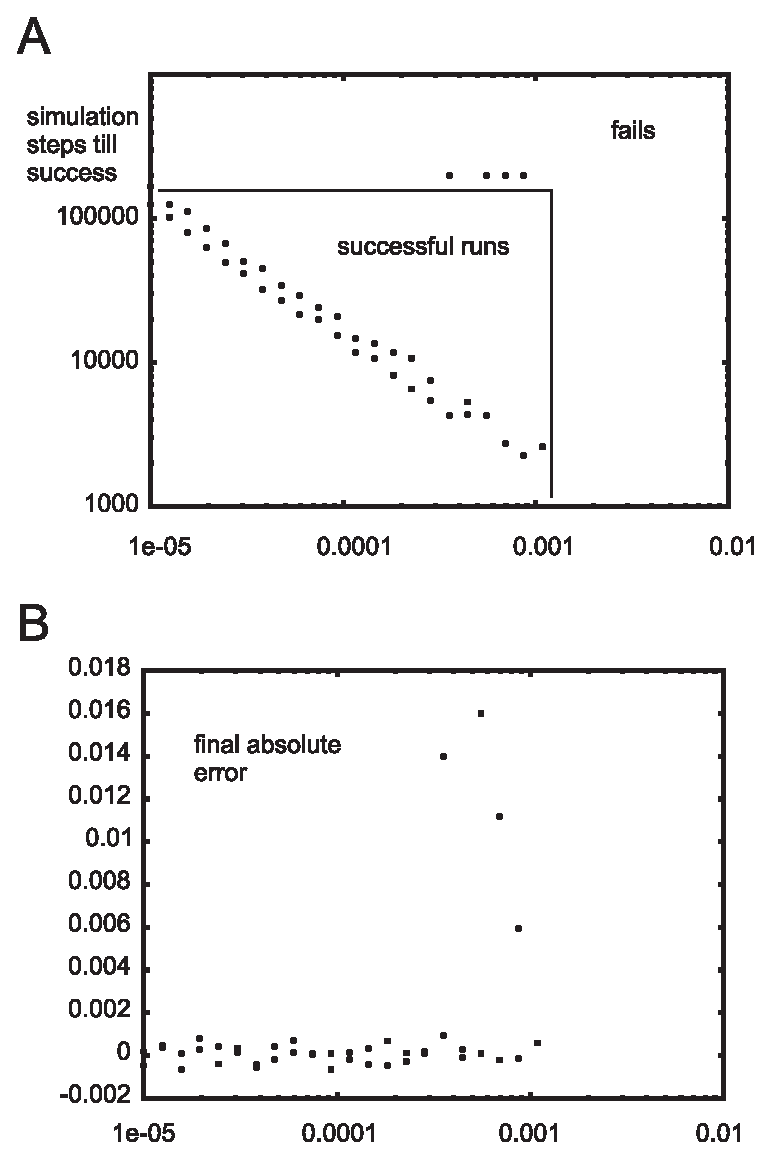
\includegraphics[width=0.9\columnwidth]{line_stats}
  \caption{Statistics of the line following task. A) shows the relation between
    'time to success' and learning rate. For every learning rate two runs have
    been conducted with different random number seeds to test the dependence on the
    initialisation of the weights. The simulation was marked successful if the
    absolute value of the error Eq.~\ref{line_abserr} stayed below $0.001$ for more than $1000$
    timesteps. The simulation was aborted after $200,000$ time steps if this criterion
    hasn't been reached. Inside of the square every run has been successful.
    B) shows the final absolute error for different learning rates.
    \label{line_stats}}
\end{figure}


We have run statistics of the line follower where we varied the
learning rate over three orders of magnitudes, and evaluated how long
it takes to stay below the error threshold for a specified time
(Fig.~\ref{line_stats}A), and the resulting absolute value of the
error (Fig.~\ref{line_stats}B). The time to reach the criterion
decreases with higher learning rates, and is stable up to a learning
rate of approx $\gamma = 0.001$ with no failures below a learning rate of
$\gamma = 0.0002$. Each simulation was run twice with two different random seeds to
test for initialisation effects -- it can clearly be seen that
the seed has an effect on both the number of simulation steps,
and at higher learning rates the final error, which is in agreement with other neural
network architectures that initialisation matters.


\begin{figure*}[!ht]
	\centering 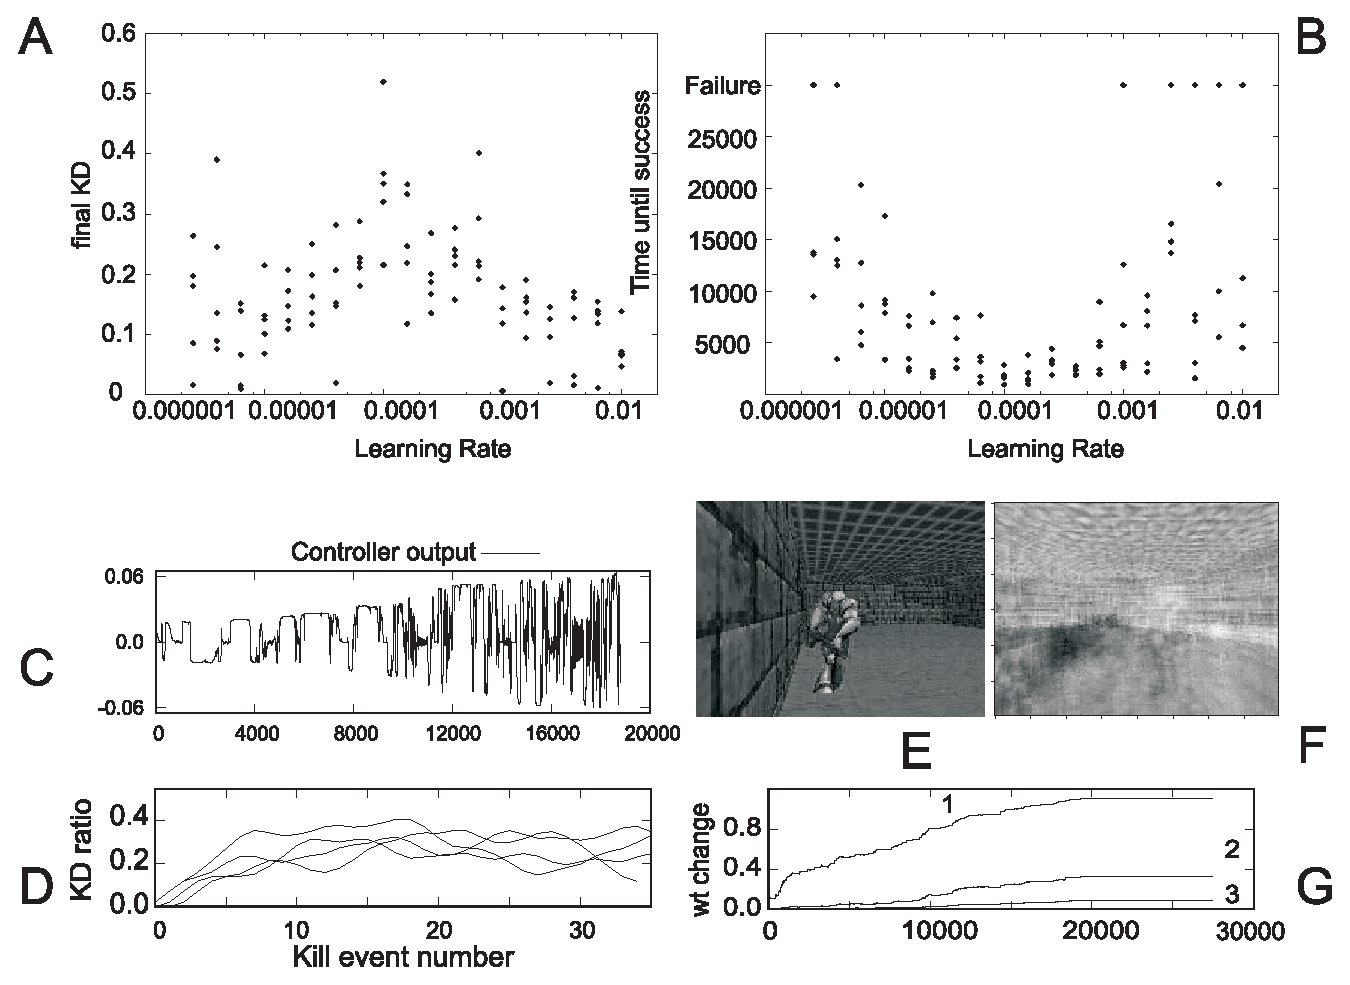
\includegraphics[width=0.9\textwidth]{FPSFig4}
	\caption{A) KD at end of trial. B) Time to success vs learning
          rate - success is if the smoothed KD ratio reaches a
          threshold of 0.15. C) $\Delta \theta$, the rate of change in
          bot's orientation against simulation step number, purely
          from the DFL output, in arbitrary units. D) KD learning
          curves - the time series of kills/deaths is filtered with a
          2nd order lowpass filter to get a moving average, plotted
          against kill event number. E) Example input frame. F) Example input weights. G) Euclidean distance of weights
          for each layer from their initial point, against learning
          step. 
          Parameters: 19200 inputs from grayscale image; 2
          hidden layers of 5 units each; no filterbank. Inputs were
          normalised to zero-mean, unit variance. Learning rate in D
          and E was 0.0001.
		\label{shooter_results}}
\end{figure*}




\section{Shooter game}
In this scenario, we try to learn to play a first-person shooter
purely from visual inputs. We use the Vizdoom
(http://vizdoom.cs.put.edu.pl/) environment for this purpose, and
train a controller to play against a single pre-trained bot from Intel
that ran in the Vizdoom 2016 competition. The setup was as follows:

The images returned from Vizdoom are RGB 160x120. We rendered the
enemy in blue, and formed a reflex signal by finding the bounding box
of the pixels closest to that colour. Note that the reflex is slow and
also inherently noisy, as other events in the game are also rendered
blue (e.g. the 'flashes' that happen at respawns). The reflex also
fails at times when the enemy is too distant or too close to the
camera. For learning, we only supply the network with the greyscale
image (Fig.~\ref{shooter_results}G) flattened into a vector of $19200$
inputs, so it is forced to discover purely spatial cues. The reflex is
computed relative to the image centre, so a negative value implies the
enemy is on the left. Shooting behaviour is entirely hardwired: if an
enemy is detected within a certain distance of the image centre, the bot
fires. Note that the bot's only actions are to rotate in the plane,
and shoot -- it does not translate in the environment (the enemy moves freely). Instead of
separate outputs for left and right, we have a single value produced
by 3 neurons acting at different sensitivities:
\begin{equation}
\Delta \theta = g_{err}\, \mathrm{error} + g_{net} \left( 10 v_0 + 3 v_1 + v_2 \right)
\end{equation}
where $v_0, \ldots, v_2$ are the network outputs, and $\Delta \theta$
is the change in orientation.


\subsection{Results}
As before, we see that the controller outputs steadily increase over
time (Fig.~\ref{shooter_results}C). With a high value of $g_{net}$,
the bot can make very rapid aiming movements. This has the advantage
that the error can in principle be reduced very quickly; it also
causes the bot to sometimes make large rotations even when the enemy
is out of the field of view, which helps with exploration. On the
other hand, it can cause the aiming to overshoot and oscillate around
the target.  The weights grow in a similar pattern to before, although
their progression is less smooth, due to the more discontinuous nature
of the error signal (Fig.~\ref{shooter_results}E). The different
scales are likely due to the inputs having more dimensions.

Unlike the Line Follower the error signal has high transients as there
are discontinuities when the bot respawns and the enemy will often
appear unpredictably somewhere in the image. Instead of averaging over
long periods of time to test if the error signal is converging we
simply measure how often our bot is killed vs how often it kills the
enemy. In gaming, this is called the kill/death ratio, and we plot
some smoothed KD curves in Fig.~\ref{shooter_results}D. To do
statistics, we measure the time taken to reach a threshold KD of 0.15
- Fig.~\ref{shooter_results}B shows this as a function of learning
rate. As before, there is a stable region in the middle where learning
is consistently successful. We also plot the smoothed KD for the final
step of each trial(Fig.~\ref{shooter_results}A); although a noisy
performance measure, the same pattern emerges. Over time, the input
weights blur the background, leaving dark and light blobs to detect
the enemy and generate an aiming response
(Fig.~\ref{shooter_results}F).

Note that this is only one skill of a functioning FPS bot, as a real
bot would require additional skills such as seeking rewards
(e.g. finding health packs) and navigating the environment
(e.g. avoiding collisions). Future research will investigate whether
the DFL approach can be used to acquire such skills by applying it to
not only reflex based learning but also to other error driven
approaches. For example, one could use the reward prediction
error from TD learning and feed it into the DFL network.


\section{Discussion}
We have shown that a deep network which propagates its errors in a forward
fashion from its inputs to its outputs is able to solve closed loop
learning tasks. We have demonstrated this in both a first person
shooter and a driving scenario.

Closed loop learning which aims to maximise a function or minimise one
is usually referred to as reinforcement learning, where an agent learns to
navigate an action space in a way that it maximises its accumulative
reward \cite{Dayan1992,Abbott01}. The main drawback of this approach
is the discrete state space which makes it hard to solve analogue
problems. To overcome this problem, closed loop learning rules using
correlation-based techniques \cite{Verschure91} were introduced.
These networks perform well in real robot tasks but are usually restricted to 
simple network architectures. DFL addresses this
deficiency by introducing a deep architecture but staying firmly
on correlation-based territory.

Plasticity has always been hotly debated in neurophysiology -- the
general understanding is that a large postsynaptic Calcium
concentration causes LTP \cite{Malenka99,Bennett2000} and a low one
causes LTD \cite{Mulkey1992}. This requires a strong pre-synaptic
drive to achieve a strong postsynaptic activity, and with that Ca
influx \cite{Meunier2017}. In mathematical terms this would just lead
to self-amplification of the synaptic weight, where strong presynaptic
activity would lead to more postsynaptic activity and in turn stronger
weights, and so on. However, suppose the learning signal and the
actual activity were transmitted via the same synapse but were
fundamentally separated \cite{Lindsay2017}, for example by using
different frequencies: high frequency potentials could cause
plasticity changes while low frequency potentials propagate
behaviourally relevant activity \cite{Canolty2010}. DFL would provide
here a mechanism which allows stable behaviourally-relevant learning
driven by heterosynaptic plasticity and Hebbian learning for the error
signal; the stability arising from the fact that it is constantly
corrected by the error signal.

Looking at a system-wide perspective, one can see DFL as a flexible
actor which has a high degree of freedom in generating actions as long as they
minimise the error. For example in the basal ganglia the striatum is
seen as an actor receiving an error signal via dopamine, the famous
reward prediction error \cite{Schultz97} which is understood as being
closely related to the error of temporal difference learning
\cite{gurney98:_basal_gangl_action_selec_devic}. It is curious that
the striatum receives the error signal but both downstream neurons in
the basal ganglia and upstream in the cortex receive little
dopaminergic modulation \cite{Beckstead1979}. However, plasticity is
not just limited to the striatum, but happens in all brain areas, so
it makes sense to propagate this further back into the cortex
\cite{Groenewegen1993} where high level decision-making takes place.
Coming back to classical TD learning \cite{Sutton87}, which is
certainly a perfect match for striatal decision making, one can see
deep feedback learning in this context as an actor which receives an
error signal from a critic. In a biological context this error signal
could indeed then feed into the striatum initially as dopamine, but
then when fed back into the cortex would propagate as activity
as well and not just neuromodulation, using cross frequency coupling
as described above \cite{Lipski2017}.

Given that in DFL the error is propagated from the input to the
output, the novel aspect is that the more layers DFL has, the more it
is remote from the immediate error feedback. This allows for
a flexibility which is a function of the number of layers, and
creates an actor which is far less rigid than a standard Q learning
actor \cite{Dayan1992}. The actions can be substantially varied as
long as the error signal can be minimised, and the variability will be
more pronounced with more hidden layers. In other words the more
hidden layers we have the more behavioural flexibility the agent will
show.

A different stance about synaptic plasticity (and ultimately how
autonomous agents learn) has been taken by the deep learning
community, which has recently claimed that error backpropagation is
biologically realistic \cite{Lillicrap2016,Roelfsema2018}. This has
been demonstrated in a network with one hidden layer by introducing a
separate feedback pathway from the output of the network to this
hidden layer; this does not take account the above mentioned
cortico-striatal network. While this shows promising results for
abstract models of biologically motivated decision making it still
operates in an open loop fashion (i.e. output control), and thus
contradicts the requirement for an agent to control its inputs.

Autonomous behaviour can only be understood by observing the whole
loop \cite{Porr2005kyb}, be it reinforcement learning \cite{Sutton98}
or correlation based learning \cite{Verschure91}. Of course not all
feedback loops traverse through the physical environment; they could
be efference copies \cite{Uexkuell26,Graesser86}, gating signals or
mental processes. However, even these signals need to be evaluated at
the input of the agent, for example when stabilising an input image,
the goal is itself an image, and therefore an input and not an output.

\bibliographystyle{abbrv}

\bibliography{hebb,ours,embodiment,laplace,limbic,selbstorg}

\end{document}
